\documentclass[9pt, addpoints]{exam}
\usepackage[english]{babel}
\usepackage[utf8x]{inputenc}
\usepackage{graphicx,lastpage}
\usepackage{hyperref}
\usepackage{amsmath}
\usepackage{amsthm}
\usepackage{amsfonts}
\usepackage{amssymb}
\usepackage{scrextend}
\usepackage{mathrsfs}
\usepackage{hhline}
\usepackage{booktabs} % book-quality tables
\usepackage{units}    % non-stacked fractions and better unit spacing
\usepackage{multicol} % multiple column layout facilities
\usepackage{lipsum}   % filler text
\usepackage{varwidth} % centering for itemize
\usepackage{listings}
\usepackage[linewidth=1pt]{mdframed}

\renewcommand{\qedsymbol}{$\blacksquare$}

\qformat{\thequestion\dotfill \emph{\totalpoints\ points}}
\pagestyle{headandfoot}
\header{T-409-TSAM}{Assignment 4}{\thepage/\numpages}
\runningheadrule
\firstpagefooter{}{}{}
\runningfooter{}{Page \thepage\ of \numpages}{}

\graphicspath{{.}}
\printanswers

\title{Assignment 4}

\begin{document}
\noindent
\begin{minipage}[l]{.11\textwidth}%
\noindent
    
\includegraphics[width=\textwidth]{HR}
\end{minipage}%
%\hfill
\begin{minipage}[r]{.6\textwidth}%
\begin{center}
    {\large\bfseries Department of Computer Science \par
    \large Computer Networks \\[2pt]
    \large Due: Sunday 27th October (23.59)
    }
\end{center}
\end{minipage}%
\fbox{\begin{minipage}[l]{.4\textwidth}%
\noindent
    {\bfseries Your name:}\\[2pt]
TA Name:    \\
Time Taken: \\
{\footnotesize Estimated Time: {20 hours}}
\end{minipage}}%
\large     
\vspace{2cm}
\begin{center}
    \begin{minipage}{40em}
        \vspace{6pt}
        \begin{center}
            \textbf{This is a paired assignment - you may choose to work with one other
            person if you wish, and submit the assignment together.}
        \end{center}
        \vspace{6pt}

        This assignment can be submitted as a pdf using 
        Canvas.  For those who like to dabble in the dark arts, the latex version 
        is also available, but you may submit in any legible form you wish.
        Marks are awarded for question difficulty. While there is 
        typically a relationship between difficulty and length of answer,
        it may not be a strong one. 
        \\
        \\
        \textbf{Explain your answer or give full derivation
        of results where appropriate. Solitary solutions without explanation
        risk receiving 0 points, even when correct. In particular if there are
        2 points for a short question, 1 of them will be for the explanation.}
        \vspace{12pt}
        \\
        Optional: Please include a rough estimate of how long it took you do the 
        assignment so that we can calibrate the work being assigned for the 
        course. (The estimated time is provided purely as a guideline.)
        \par
        \vspace{12pt}
    \end{minipage}
\end{center}
\vspace{4cm}

\begin{center}
    \gradetable[h]
\end{center}
\newpage

\begin{questions}
\section*{Network Trivia}
\question

\begin{parts}
\part[2] What is a Media Access Control(MAC) Address? 

\vspace{\stretch{1}}
\part[2] How does Wireshark know the manufacturer of the device sending a packet?

\vspace{\stretch{1}}
\part[2] Why is a random interval added to the CSMA backoff and try again protocol?

\vspace{\stretch{1}}
\part[2] Why is it a good idea to keep the size of individual messages sent across
the open Internet to less than 1450 bytes?

\vspace{\stretch{1}}
\part[2] What is an open DNS amplification attack?

\vspace{\stretch{1}}
\part[2] What is an Autonomous System(AS) and how are they identified as part 
of the internet.

\vspace{\stretch{1}}
\part[2] Where are the routing tables for the backbone routers of the Internet calculated?

\vspace{\stretch{1}}
\part[2] What is the Internet Control Message Protocol (ICMP) used for?

\vspace{\stretch{1}}
\part[2] Why is it ill-advised to look directly into the end of a fibre optic cable?

\vspace{\stretch{1}}
\part[3] Explain the differences between symmetric and asymmetric encryption?
\vspace{\stretch{1}}

\part[2] Why is flow control important at all levels of the network stack?

\end{parts}
\newpage
\section*{Queuing Theory}

\question
\begin{parts}
    \part[4] In the Kendall Queuing System Notation (X/X/x/X), what do the first four
    terms stand for?

\vspace{\stretch{1}}
    \part
        An IT help desk is available 8 hours a day, with a single person to 
        provide help. Assume the average
        exponentially distributed service time for each person needing help 
        is 10 minutes, and there are 4 arrivals an hour.

 
    \begin{subparts}  
        \subpart[3] How long on average will each person have to wait in the queue?
\vspace{\stretch{1}}

        \subpart[3] How many IT specialists will need to be provided to prevent
        anybody queueing?
\vspace{\stretch{1}}

        \subpart[2] What critical assumption does the answer to part ii depend on?
\vspace{\stretch{1}}

        \subpart[2] At what particular time of the day is this assumption likely
        to be incorrect?
\vspace{\stretch{1}}
    \end{subparts}
\end{parts}
\newpage
\section*{Information Theory}
\question
\begin{parts}
\part[4] Shannon's limit on the communication of information in a single
        channel, places a hard mathematical limit on the amount of information
        that can be communicated over a single channel for a given amount
        of bandwidth, power and noise.  Consider 5 devices that are connected
        via copper wires, versus 5 devices that are connected via WiFi.
        Assume that the bandwidth, power, and noise of the communication medium
        (i.e. copper vs wireless) are identical.

        Is the amount of information that can be transmitted to the end devices
        the same in both scenarios? Explain.

\vspace{\stretch{1}}


\part You are asked to audit a real time networked system, with a full
mesh topology.  Each node in the system can receive and process 100 messages/second
from other nodes in the system. What is the maximum number of nodes the
system can support, when:
    \begin{subparts}
        \subpart[2] On receipt of any message, a node sends a message to at most one other node
        in the mesh.

        \subpart[2] On receipt of any message, a node sends a message to all the other nodes in
        the mesh.

        \subpart[2] Pick one of the two cases above, and explain how it could be
        re-architected to have more nodes than the limit you calculated.
    \end{subparts}

\vspace{\stretch{1}}

\end{parts}

\newpage
\section*{TCP/IP}
\question
  \begin{parts}
      \part[3] The table below shows the sequence of events that happen during a TCP connections      between two hosts A and B, when A opens a connectiion to B, sends a single data segment, 
      and then closes the connection. Order the events as they
      occur as part of the connection, and indicate which host or hosts they occur at.

      \begin{tabular}{|p{1cm}|p{1cm}|p{2cm}|c|}
      \hline
      Order & A & B   & Event \\
      \hline
            &   &     & Send an ACK segment         \\
      \hline
            &   &     & Do the rest of the data exchange         \\
      \hline
            &   &     & Close the connection         \\
      \hline
            &   &     & Send an ACK segment         \\
      \hline
            &   &     & Send a FIN segment         \\
      \hline
            &   &     & Send a SYN segment         \\
      \hline
            &   &     & Send a FIN segment         \\
      \hline
            &   &     & Send a SYN-ACK segment         \\
      \hline
            &   &     & Enter the TIME-WAIT state         \\
      \hline
            &   &     & Send an ACK+DATA segment         \\
      \hline
            &   &     & Close the connection         \\
      \hline
      \end{tabular}

      \part[2] Draw a labelled diagram of the three part opening handshake
      of a TCP/IP connection, showing the sequence, acknowledgement values
      and type of each segment sent.
\vspace{\stretch{1}}

      \part[2] What is the purpose of a SYN cookie?
\vspace{\stretch{1}}

      \part[2] What guarantee does TCP/IP provide for connections which are made using it?
\vspace{\stretch{1}}

      \part[2] What is the advantage of TCP Selective Acknowledgements (SACK) over
      the original cumulative acknowledgement scheme?
\vspace{\stretch{1}}

      \part[2] What is silly window syndrome?
\vspace{\stretch{1}}
  \end{parts}

  \newpage
\section*{Networks and Addressing}
\question
  \begin{parts}
     \part[3] For each of the following subnet addresses, provide the range of
     of IP Addresses that can be assigned to that subnet, and the broadcast 
     address for that subnet.  

      \begin{table}[ht]
          \centering
         \begin{tabular}{|l|l|l|}
             \hline
     Subnet  & IP Address Range in the Subnet  & Broadcast address \\
             \hline
                    &        &    \\
     44.36.35.0/27  &        &    \\
                    &        &    \\
                    &        &    \\
                    \hline
                    &        &    \\
     10.12.13.0/24  &        &    \\
                    &        &    \\
                    &        &    \\
                    \hline
                    &        &    \\
     18.0.0.0/8     &        &    \\
                    &        &    \\
                    &        &    \\
             \hline
         \end{tabular}
     \end{table}

    \part[2] What addressing problem does Network Address Translation(NAT) solve
    for IPv4 network addresses?
\vspace{\stretch{2}}

     \part[3] Because NAT violates the end to end principle of the Internet,
     initiating connections to addresses behind NAT routers is problematic.
     Name one of the techniques that can be used used to  overcome this problem,
     and briefly describe how it works.
\vspace{\stretch{2}}
  \end{parts}
\newpage
\section*{Network Design and Security}
\question
You have been asked to consult on the network security of the small health
clinic shown in the diagram below. All computers in the clinic are on the
same Local Area Network(LAN), which uses a small cisco router to connect
to the Internet. The medical record database is stored on a dedicated linux computer
also on the LAN, and is accessed by all the office computers except the payroll
computer. A WiFi Network is used by employees to access the LAN
with their cell phones, and to provide a guest network for patients. The fishtank
is not on any network, but a manufacturer supplied cellphone APP is used to
monitor its temperature by staff.

The clinic also supports a public web server which is used
for patient appointments, to advertise times for Flu shots and other
public announcements.

\begin{figure}[ht]{}
  \centering
  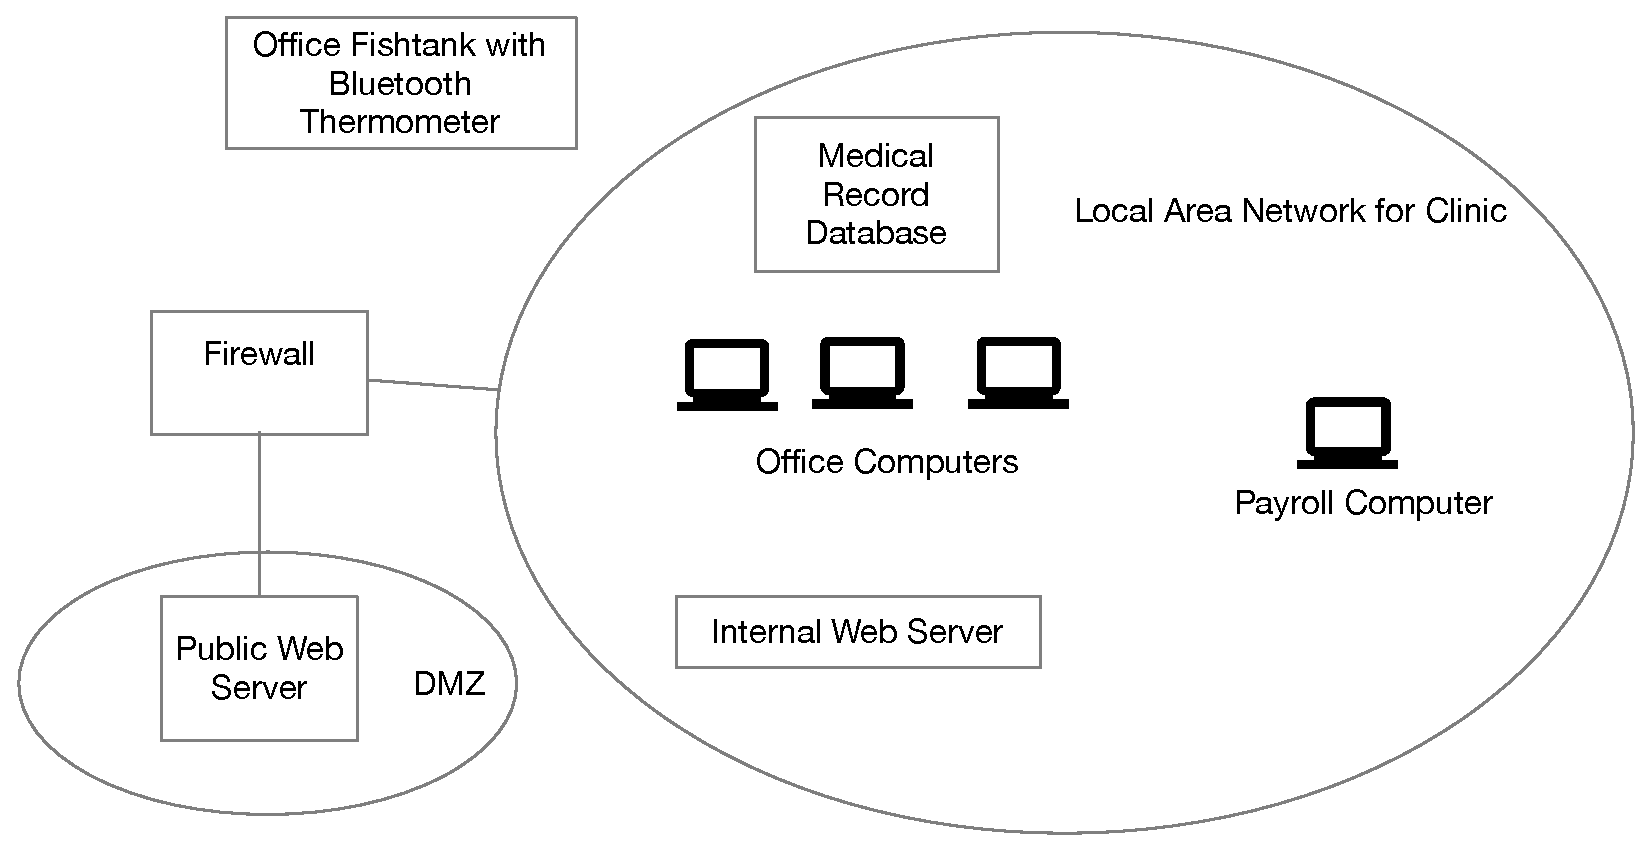
\includegraphics[width=10cm]{lan}
\end{figure}

\begin{parts}
\part[2] What is the purpose of the Demilitarized Zone(DMZ)?
\vspace{\stretch{1}}
\part[2] Is one firewall sufficient? 
\vspace{\stretch{1}}

\part[4] The clinic's WWW address was recently used in a phishing attack,
after attackers altered its public DNS record via a DNS cache poisoning exploit.
Explain what happened, and how the clinic could prevent this from happening again.
\vspace{\stretch{1}}

\part The Blueborne(CVE-2017-1000251) attack, announced in September 2017, allows an
attacker to install and run malicious code on affected bluetooth devices without any interaction
with the user. The attack has been sucessfully demonstrated on all major computer and mobile
phone platforms, and many other bluetooth devices.  The attack can also propagate itself 
to other bluetooth devices.

Assume that none of the Bluetooth devices in the Clinic have been patched.
\begin{subparts}
    \subpart[2] Explain how an attacker on the Guest network could probe for local bluetooth
devices.
\vspace{\stretch{1}}

\subpart[4] Explain all the steps in a plausible attack that uses the office fishtank
to attack the payroll computer and extract data to a visitor's laptop.
\vspace{\stretch{3}}

\end{subparts}

\part[4] Given that the Cisco router provides support for Virtual Lans (VLAN),
draw and label a diagram showing how to reorganise the network to provide better security for
the payroll computer. You may add additional named devices if you wish, and should provide
a brief explanation for the reasons for your changes. 

\end{parts}

\section*{Bluetooth}
\question
\begin{parts}
\part An American company is selling a personalised, Bluetooth 5.0 toothbrush,
which measures heartrate, brushing frequency, and duration of brushing. It uploads
this information to a company server. The
product is marketed specifically towards children, under the age of 12, to help
their parents monitor their brushing habits. The devices use a commodity chip
which supports the full bluetooth stack, and pairs with an Android phone acting
as a master.
\begin{subparts}
\subpart[2] What is the bluetooth Generic Access profile(GAP)?
\vspace{\stretch{1}}
\subpart[2] Explain how two Bluetooth LE devices from different manufacturers
can share information.
\vspace{\stretch{2}}
\subpart[2] How will the toothbrushes pair with a phone?
\vspace{\stretch{1}}

\subpart[4] The company also sells a blue tooth enabled smart lightbulb, which is controlled
with the same software. A household using both products will typically have
over 20 light bulbs and several toothbrushes.

Describe using a labelled diagram, and stating clearly any restrictions on connectivity,
how these bluetooth 5.0 devices can network together.
\vspace{\stretch{2}}
\subpart[4] A large number of dentists have been given these toothbrushes as part of a marketing campaign to
distribute to customers. Unknown to either the dentists or the manufacturer, hackers have
found a way to use the firmware in the toothbrushes to create a botnet for industrial espionage. Describe a
plausible way this could be done, assuming that each household has at least
one mobile phone which has not been updated to fix the Blueborne attacks.
Include an explanation of how the toothbrushes could be identified, and also how
information can be extracted from the toothbrushes back to Hacker HQ.
\end{subparts}

\end{parts}

\end{questions}
\end{document}
